% Generated by scripts/analysis/render_poster_matrices.py (information).
% source_csv_sha256=bffb8776b7c15ecdee40e8de6b8b80c726e05d5be065b54a309b8e8bc9d9b5c2
% source_csv=/Users/rasikaramanan/Documents/usc/by_semester/f26/csci566/project/synthea-prep/experiments/results_all_variants/experiment_results.csv
\documentclass[border=2pt]{standalone}
\usepackage[T1]{fontenc}
\usepackage[scaled=0.95]{helvet}
\renewcommand{\familydefault}{\sfdefault}
\usepackage{tikz}
\ifdefined\pdfinfoomitdate\pdfinfoomitdate=1\fi
\ifdefined\pdftrailerid\pdftrailerid{}\fi
\begin{document}
\begin{minipage}{16cm}
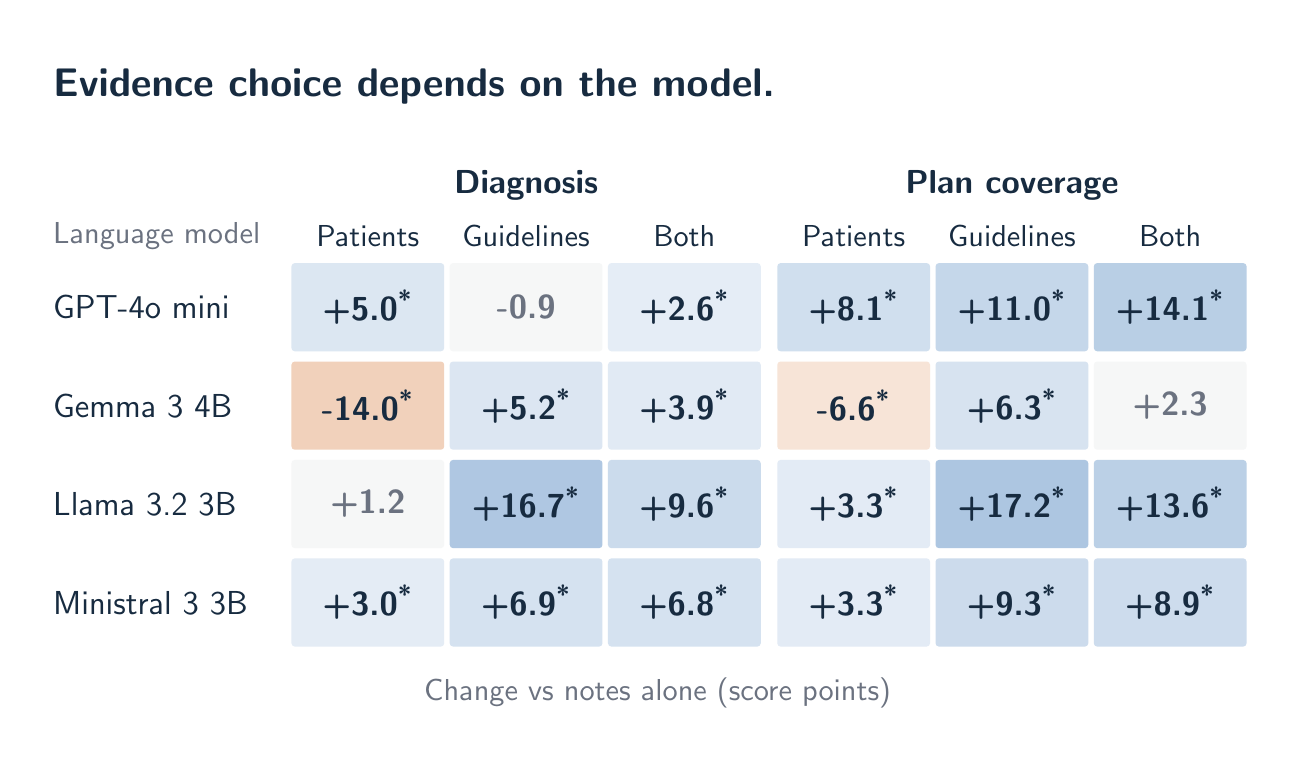
\begin{tikzpicture}[x=1cm,y=1cm]
\definecolor{matrixink}{HTML}{172B40}
\definecolor{matrixmuted}{HTML}{6B7280}
\definecolor{matrixpositive}{HTML}{3E79B8}
\definecolor{matrixnegative}{HTML}{D98042}
\useasboundingbox (0,0) rectangle (16,9);
\fill[white] (0,0) rectangle (16,9);
\node[anchor=west,text=matrixink,font=\fontsize{15}{18}\selectfont\bfseries] at (0.2,8.25) {Evidence choice depends on the model.};
\node[anchor=west,text=matrixmuted,font=\fontsize{10.5}{12}\selectfont] at (0.2,6.36) {Language model};
\node[text=matrixink,font=\fontsize{12}{14}\selectfont\bfseries] at (6.330,7.0) {Diagnosis};
\node[text=matrixink,font=\fontsize{10.5}{12}\selectfont] at (4.320,6.36) {Patients};
\node[text=matrixink,font=\fontsize{10.5}{12}\selectfont] at (6.330,6.36) {Guidelines};
\node[text=matrixink,font=\fontsize{10.5}{12}\selectfont] at (8.340,6.36) {Both};
\node[text=matrixink,font=\fontsize{12}{14}\selectfont\bfseries] at (12.500,7.0) {Plan coverage};
\node[text=matrixink,font=\fontsize{10.5}{12}\selectfont] at (10.490,6.36) {Patients};
\node[text=matrixink,font=\fontsize{10.5}{12}\selectfont] at (12.500,6.36) {Guidelines};
\node[text=matrixink,font=\fontsize{10.5}{12}\selectfont] at (14.510,6.36) {Both};
\node[anchor=west,text=matrixink,font=\fontsize{11.5}{14}\selectfont] at (0.2,5.450) {GPT-4o mini};
% cell model=gpt_4o_mini metric=diagnosis source=patient_retrieval baseline_variant=llm_only comparison_variant=patient_retrieval n_pairs=2378 n_patients=2047 mean_baseline=0.7582558630072681 mean_comparison=0.8086805609827662 mean_difference=0.050424697975498 p_value_two_sided=8.765318235532143e-37 p_value_two_sided_holm=3.418474111857536e-35
\fill[matrixpositive!18.08,rounded corners=1.2pt] (3.350,4.890) rectangle (5.290,6.010);
\node[text=matrixink,font=\fontsize{13}{15}\selectfont\bfseries] at (4.320,5.450) {+5.0\textsuperscript{*}};
% cell model=gpt_4o_mini metric=diagnosis source=guidelines baseline_variant=llm_only comparison_variant=guidelines n_pairs=2378 n_patients=2047 mean_baseline=0.7582558630072681 mean_comparison=0.7491430917039282 mean_difference=-0.00911277130334 p_value_two_sided=0.0184109870418573 p_value_two_sided_holm=0.2577538185860024
\fill[matrixink!4,rounded corners=1.2pt] (5.360,4.890) rectangle (7.300,6.010);
\node[text=matrixmuted,font=\fontsize{13}{15}\selectfont\bfseries] at (6.330,5.450) {-0.9};
% cell model=gpt_4o_mini metric=diagnosis source=both baseline_variant=llm_only comparison_variant=patient_retrieval_guidelines n_pairs=2378 n_patients=2047 mean_baseline=0.7582558630072681 mean_comparison=0.7846751997489514 mean_difference=0.0264193367416831 p_value_two_sided=1.0217930926367319e-10 p_value_two_sided_holm=2.963199968646522e-09
\fill[matrixpositive!13.28,rounded corners=1.2pt] (7.370,4.890) rectangle (9.310,6.010);
\node[text=matrixink,font=\fontsize{13}{15}\selectfont\bfseries] at (8.340,5.450) {+2.6\textsuperscript{*}};
% cell model=gpt_4o_mini metric=plan source=patient_retrieval baseline_variant=llm_only comparison_variant=patient_retrieval n_pairs=2271 n_patients=1967 mean_baseline=0.294840745633348 mean_comparison=0.375348598268017 mean_difference=0.080507852634669 p_value_two_sided=6.367765766341893e-20 p_value_two_sided_holm=1.974007387565987e-18
\fill[matrixpositive!24.10,rounded corners=1.2pt] (9.520,4.890) rectangle (11.460,6.010);
\node[text=matrixink,font=\fontsize{13}{15}\selectfont\bfseries] at (10.490,5.450) {+8.1\textsuperscript{*}};
% cell model=gpt_4o_mini metric=plan source=guidelines baseline_variant=llm_only comparison_variant=guidelines n_pairs=2267 n_patients=1964 mean_baseline=0.2947728275253639 mean_comparison=0.4048669313336274 mean_difference=0.1100941038082635 p_value_two_sided=4.965237832201895e-44 p_value_two_sided_holm=2.0853998895247958e-42
\fill[matrixpositive!30.02,rounded corners=1.2pt] (11.530,4.890) rectangle (13.470,6.010);
\node[text=matrixink,font=\fontsize{13}{15}\selectfont\bfseries] at (12.500,5.450) {+11.0\textsuperscript{*}};
% cell model=gpt_4o_mini metric=plan source=both baseline_variant=llm_only comparison_variant=patient_retrieval_guidelines n_pairs=2269 n_patients=1967 mean_baseline=0.2946966358160717 mean_comparison=0.4353973850448068 mean_difference=0.1407007492287351 p_value_two_sided=4.057924842065906e-62 p_value_two_sided_holm=1.7854869305089986e-60
\fill[matrixpositive!36.14,rounded corners=1.2pt] (13.540,4.890) rectangle (15.480,6.010);
\node[text=matrixink,font=\fontsize{13}{15}\selectfont\bfseries] at (14.510,5.450) {+14.1\textsuperscript{*}};
\node[anchor=west,text=matrixink,font=\fontsize{11.5}{14}\selectfont] at (0.2,4.200) {Gemma 3 4B};
% cell model=ollama_gemma3_4b metric=diagnosis source=patient_retrieval baseline_variant=llm_only comparison_variant=patient_retrieval n_pairs=2378 n_patients=2047 mean_baseline=0.6411567751812953 mean_comparison=0.5009275054438571 mean_difference=-0.1402292697374382 p_value_two_sided=1.8246914922638968e-103 p_value_two_sided_holm=8.393580864413926e-102
\fill[matrixnegative!36.05,rounded corners=1.2pt] (3.350,3.640) rectangle (5.290,4.760);
\node[text=matrixink,font=\fontsize{13}{15}\selectfont\bfseries] at (4.320,4.200) {-14.0\textsuperscript{*}};
% cell model=ollama_gemma3_4b metric=diagnosis source=guidelines baseline_variant=llm_only comparison_variant=guidelines n_pairs=2378 n_patients=2047 mean_baseline=0.6411567751812953 mean_comparison=0.6930979325668635 mean_difference=0.051941157385568 p_value_two_sided=2.2319174616735117e-22 p_value_two_sided_holm=7.365327623522589e-21
\fill[matrixpositive!18.39,rounded corners=1.2pt] (5.360,3.640) rectangle (7.300,4.760);
\node[text=matrixink,font=\fontsize{13}{15}\selectfont\bfseries] at (6.330,4.200) {+5.2\textsuperscript{*}};
% cell model=ollama_gemma3_4b metric=diagnosis source=both baseline_variant=llm_only comparison_variant=patient_retrieval_guidelines n_pairs=2378 n_patients=2047 mean_baseline=0.6411567751812953 mean_comparison=0.6799438754506545 mean_difference=0.0387871002693592 p_value_two_sided=1.4056251614600718e-10 p_value_two_sided_holm=3.935750452088201e-09
\fill[matrixpositive!15.76,rounded corners=1.2pt] (7.370,3.640) rectangle (9.310,4.760);
\node[text=matrixink,font=\fontsize{13}{15}\selectfont\bfseries] at (8.340,4.200) {+3.9\textsuperscript{*}};
% cell model=ollama_gemma3_4b metric=plan source=patient_retrieval baseline_variant=llm_only comparison_variant=patient_retrieval n_pairs=2265 n_patients=1959 mean_baseline=0.2207873436350257 mean_comparison=0.1552244297277409 mean_difference=-0.0655629139072847 p_value_two_sided=7.669311366079993e-22 p_value_two_sided_holm=2.454179637145597e-20
\fill[matrixnegative!21.11,rounded corners=1.2pt] (9.520,3.640) rectangle (11.460,4.760);
\node[text=matrixink,font=\fontsize{13}{15}\selectfont\bfseries] at (10.490,4.200) {-6.6\textsuperscript{*}};
% cell model=ollama_gemma3_4b metric=plan source=guidelines baseline_variant=llm_only comparison_variant=guidelines n_pairs=2270 n_patients=1964 mean_baseline=0.2217694566813509 mean_comparison=0.2847650513950073 mean_difference=0.0629955947136563 p_value_two_sided=3.7858309023613585e-17 p_value_two_sided_holm=1.1357492707084078e-15
\fill[matrixpositive!20.60,rounded corners=1.2pt] (11.530,3.640) rectangle (13.470,4.760);
\node[text=matrixink,font=\fontsize{13}{15}\selectfont\bfseries] at (12.500,4.200) {+6.3\textsuperscript{*}};
% cell model=ollama_gemma3_4b metric=plan source=both baseline_variant=llm_only comparison_variant=patient_retrieval_guidelines n_pairs=2275 n_patients=1968 mean_baseline=0.2221611721611721 mean_comparison=0.2451282051282051 mean_difference=0.0229670329670329 p_value_two_sided=0.0023568162095285 p_value_two_sided_holm=0.0377090593524565
\fill[matrixink!4,rounded corners=1.2pt] (13.540,3.640) rectangle (15.480,4.760);
\node[text=matrixmuted,font=\fontsize{13}{15}\selectfont\bfseries] at (14.510,4.200) {+2.3};
\node[anchor=west,text=matrixink,font=\fontsize{11.5}{14}\selectfont] at (0.2,2.950) {Llama 3.2 3B};
% cell model=ollama_llama3_2_3b metric=diagnosis source=patient_retrieval baseline_variant=llm_only comparison_variant=patient_retrieval n_pairs=2378 n_patients=2047 mean_baseline=0.4965511738963112 mean_comparison=0.508836536416325 mean_difference=0.0122853625200137 p_value_two_sided=0.0877005941425622 p_value_two_sided_holm=1.0
\fill[matrixink!4,rounded corners=1.2pt] (3.350,2.390) rectangle (5.290,3.510);
\node[text=matrixmuted,font=\fontsize{13}{15}\selectfont\bfseries] at (4.320,2.950) {+1.2};
% cell model=ollama_llama3_2_3b metric=diagnosis source=guidelines baseline_variant=llm_only comparison_variant=guidelines n_pairs=2378 n_patients=2047 mean_baseline=0.4965511738963112 mean_comparison=0.663828014401109 mean_difference=0.1672768405047976 p_value_two_sided=1.9277054339337063e-137 p_value_two_sided_holm=9.252986082881792e-136
\fill[matrixpositive!41.46,rounded corners=1.2pt] (5.360,2.390) rectangle (7.300,3.510);
\node[text=matrixink,font=\fontsize{13}{15}\selectfont\bfseries] at (6.330,2.950) {+16.7\textsuperscript{*}};
% cell model=ollama_llama3_2_3b metric=diagnosis source=both baseline_variant=llm_only comparison_variant=patient_retrieval_guidelines n_pairs=2378 n_patients=2047 mean_baseline=0.4965511738963112 mean_comparison=0.5924348627116007 mean_difference=0.0958836888152893 p_value_two_sided=1.1103265890685559e-41 p_value_two_sided_holm=4.441306356274224e-40
\fill[matrixpositive!27.18,rounded corners=1.2pt] (7.370,2.390) rectangle (9.310,3.510);
\node[text=matrixink,font=\fontsize{13}{15}\selectfont\bfseries] at (8.340,2.950) {+9.6\textsuperscript{*}};
% cell model=ollama_llama3_2_3b metric=plan source=patient_retrieval baseline_variant=llm_only comparison_variant=patient_retrieval n_pairs=2284 n_patients=1977 mean_baseline=0.1635288966725043 mean_comparison=0.1968768242848803 mean_difference=0.0333479276123759 p_value_two_sided=1.7793691065419293e-05 p_value_two_sided_holm=0.0003914612034392
\fill[matrixpositive!14.67,rounded corners=1.2pt] (9.520,2.390) rectangle (11.460,3.510);
\node[text=matrixink,font=\fontsize{13}{15}\selectfont\bfseries] at (10.490,2.950) {+3.3\textsuperscript{*}};
% cell model=ollama_llama3_2_3b metric=plan source=guidelines baseline_variant=llm_only comparison_variant=guidelines n_pairs=2276 n_patients=1974 mean_baseline=0.1629320445225542 mean_comparison=0.3353471001757469 mean_difference=0.1724150556531927 p_value_two_sided=1.6902101939078193e-103 p_value_two_sided_holm=7.943987911366751e-102
\fill[matrixpositive!42.48,rounded corners=1.2pt] (11.530,2.390) rectangle (13.470,3.510);
\node[text=matrixink,font=\fontsize{13}{15}\selectfont\bfseries] at (12.500,2.950) {+17.2\textsuperscript{*}};
% cell model=ollama_llama3_2_3b metric=plan source=both baseline_variant=llm_only comparison_variant=patient_retrieval_guidelines n_pairs=2279 n_patients=1976 mean_baseline=0.1633391838525669 mean_comparison=0.2994734532689776 mean_difference=0.1361342694164107 p_value_two_sided=1.8108367715517095e-55 p_value_two_sided_holm=7.78659811767235e-54
\fill[matrixpositive!35.23,rounded corners=1.2pt] (13.540,2.390) rectangle (15.480,3.510);
\node[text=matrixink,font=\fontsize{13}{15}\selectfont\bfseries] at (14.510,2.950) {+13.6\textsuperscript{*}};
\node[anchor=west,text=matrixink,font=\fontsize{11.5}{14}\selectfont] at (0.2,1.700) {Ministral 3 3B};
% cell model=ollama_ministral_3_3b metric=diagnosis source=patient_retrieval baseline_variant=llm_only comparison_variant=patient_retrieval n_pairs=2378 n_patients=2047 mean_baseline=0.5347447584407402 mean_comparison=0.5649872585216635 mean_difference=0.0302425000809233 p_value_two_sided=3.73500213539222e-07 p_value_two_sided_holm=9.33750533848055e-06
\fill[matrixpositive!14.05,rounded corners=1.2pt] (3.350,1.140) rectangle (5.290,2.260);
\node[text=matrixink,font=\fontsize{13}{15}\selectfont\bfseries] at (4.320,1.700) {+3.0\textsuperscript{*}};
% cell model=ollama_ministral_3_3b metric=diagnosis source=guidelines baseline_variant=llm_only comparison_variant=guidelines n_pairs=2378 n_patients=2047 mean_baseline=0.5347447584407402 mean_comparison=0.6037751560556226 mean_difference=0.0690303976148823 p_value_two_sided=1.273823597599382e-32 p_value_two_sided_holm=4.713147311117713e-31
\fill[matrixpositive!21.81,rounded corners=1.2pt] (5.360,1.140) rectangle (7.300,2.260);
\node[text=matrixink,font=\fontsize{13}{15}\selectfont\bfseries] at (6.330,1.700) {+6.9\textsuperscript{*}};
% cell model=ollama_ministral_3_3b metric=diagnosis source=both baseline_variant=llm_only comparison_variant=patient_retrieval_guidelines n_pairs=2378 n_patients=2047 mean_baseline=0.5347447584407402 mean_comparison=0.6023147146296377 mean_difference=0.0675699561888975 p_value_two_sided=1.5681029283640104e-28 p_value_two_sided_holm=5.4883602492740365e-27
\fill[matrixpositive!21.51,rounded corners=1.2pt] (7.370,1.140) rectangle (9.310,2.260);
\node[text=matrixink,font=\fontsize{13}{15}\selectfont\bfseries] at (8.340,1.700) {+6.8\textsuperscript{*}};
% cell model=ollama_ministral_3_3b metric=plan source=patient_retrieval baseline_variant=llm_only comparison_variant=patient_retrieval n_pairs=2304 n_patients=1997 mean_baseline=0.2915943287037036 mean_comparison=0.3250144675925925 mean_difference=0.0334201388888888 p_value_two_sided=1.6656946848699582e-05 p_value_two_sided_holm=0.00038310977752
\fill[matrixpositive!14.68,rounded corners=1.2pt] (9.520,1.140) rectangle (11.460,2.260);
\node[text=matrixink,font=\fontsize{13}{15}\selectfont\bfseries] at (10.490,1.700) {+3.3\textsuperscript{*}};
% cell model=ollama_ministral_3_3b metric=plan source=guidelines baseline_variant=llm_only comparison_variant=guidelines n_pairs=2302 n_patients=1994 mean_baseline=0.2917028670721112 mean_comparison=0.3845207066319143 mean_difference=0.092817839559803 p_value_two_sided=2.4963871827973578e-33 p_value_two_sided_holm=9.48627129462996e-32
\fill[matrixpositive!26.56,rounded corners=1.2pt] (11.530,1.140) rectangle (13.470,2.260);
\node[text=matrixink,font=\fontsize{13}{15}\selectfont\bfseries] at (12.500,1.700) {+9.3\textsuperscript{*}};
% cell model=ollama_ministral_3_3b metric=plan source=both baseline_variant=llm_only comparison_variant=patient_retrieval_guidelines n_pairs=2304 n_patients=1995 mean_baseline=0.2921006944444444 mean_comparison=0.3815827546296296 mean_difference=0.0894820601851851 p_value_two_sided=1.5487256592146416e-29 p_value_two_sided_holm=5.575412373172709e-28
\fill[matrixpositive!25.90,rounded corners=1.2pt] (13.540,1.140) rectangle (15.480,2.260);
\node[text=matrixink,font=\fontsize{13}{15}\selectfont\bfseries] at (14.510,1.700) {+8.9\textsuperscript{*}};
\node[text=matrixmuted,font=\fontsize{10.5}{12}\selectfont] at (8,0.55) {Change vs notes alone (score points)};
\end{tikzpicture}
\par\centering\vspace{1mm}
{\fontsize{8}{10}\selectfont\color{black!65}* Holm-adjusted $p<.01$ (48 comparisons).\par}
\end{minipage}
\end{document}
